\documentclass[cn,hazy,cyan,11pt,normal]{elegantnote}
\usepackage{lmodern}
\usepackage{wasysym}
\usepackage{lipsum}
\usepackage{float}
\usepackage{color}
\usepackage{tcolorbox}
\usepackage{pgfplots}
\usepackage{array}
\usepackage{amsfonts}
\usepackage{mathtools}
\usepackage{dsfont}
\usepackage{extarrows}
\usepackage{bbm}

\pgfplotsset{compat=1.18}
\tcbuselibrary{listings, skins}

\allowdisplaybreaks[4]
\newfontfamily\codefont{Consolas}
\definecolor{tairitsu}{HTML}{1f1e33}

\lstset{
    language=Python,
    basicstyle=\codefont\small,
    keywordstyle=\color{blue},
    stringstyle=\color{red},
    commentstyle=\color{gray},
    numbers=left,
    numberstyle=\tiny\color{gray},
    stepnumber=1,
    numbersep=5pt,
    backgroundcolor=\color{lightgray!20},
    frame=single,
    tabsize=4,
    captionpos=b,
    breaklines=true,
    breakatwhitespace=false,
    showspaces=false,
    showstringspaces=false,
    showtabs=false,
    columns=fullflexible,
    upquote=true,
}

\newtcblisting{code}[1][Code Example]{
    listing only,
    listing options={
        language=Python,
        basicstyle=\codefont\footnotesize,
        keywordstyle=\color{blue},
        stringstyle=\color{red},
        commentstyle=\color{gray},
        numbers=left,
        numberstyle=\tiny\color{gray},
        stepnumber=1,
        numbersep=5pt,
        backgroundcolor=\color{lightgray!20},
        frame=single,
        tabsize=4,
        captionpos=b,
        breaklines=true,
        breakatwhitespace=false,
        showspaces=false,
        showstringspaces=false,
        showtabs=false,
        columns=fullflexible,
        upquote=true,
    },
    colback=lightgray!20,
    colframe=tairitsu,
    title={#1},
}



\title{最优化算法作业4}

\author{陈文轩}

\date{\today}

\definecolor{c1}{HTML}{017eda}
\definecolor{c2}{HTML}{1f1e33}

\everymath{\displaystyle}
\newcommand*{\diff}{\mathop{}\!\mathrm{d}}
\newcommand*{\prox}{\mathrm{prox}}

\DeclareMathOperator*{\argmin}{arg\,min}
\DeclareMathOperator*{\argmax}{arg\,max}
\DeclareMathOperator*{\diag}{diag}
\DeclareMathOperator*{\Diag}{Diag}
\DeclareMathOperator*{\tr}{tr}
\DeclareMathOperator*{\dom}{dom}
\DeclareMathOperator*{\st}{s.t.\,\,}


\begin{document}

    \maketitle

    \begin{enumerate}
        \item {\color{c1}对于可逆矩阵$A$,求解如下方程的零点\[F(X)=X^{-1}-A=0\]可以得到$A^{-1}$。
            \begin{enumerate}
                \item 使用牛顿法,写出迭代公式。
                \item 实现该算法,随机生成$100\times 100$维可逆矩阵$A$,作出误差随着迭代数的收敛图像。
            \end{enumerate}

            提示:根据$DF(X)[B]=-X^{-1}BX^{-1}$,计算$DF(X)^{-1}[B]$}

            \vspace{0.5cm}\textcolor{c2}{解}

            \begin{enumerate}
                \item 记Newton法迭代格式为$X_{k+1}=X_k+\Delta X$,则$\Delta X$满足$DF(X_k)[\Delta X]=-F(X_k)$,

                即$X_k^{-1}\Delta X X_k^{-1}=X_K^{-1}-A,\Delta X=X_k-X_k AX_k$,迭代公式为$X_{k+1}=2X_k-X_k AX_k$。\vspace{0.5cm}
                \item 算法代码如下:
                    \begin{code}[Newton法代码]
import numpy as np
import matplotlib.pyplot as plt
np.random.seed(42); epsilon = 0.09
A = np.random.randn(100, 100)
while np.linalg.det(A) == 0:
    A = np.random.randn(100, 100)
A_inv = np.linalg.inv(A)
X = A_inv + np.eye(100) * epsilon
max_iter = 50; errors = []
for k in range(max_iter):
    X_new = 2 * X - np.dot(np.dot(X, A), X)
    error = np.linalg.norm(X_new - A_inv, 'fro')
    errors.append(error); X = X_new
plt.plot(range(max_iter), errors)
plt.yscale('log'); plt.xlabel('Iteration')
plt.ylabel('Frobenius Norm of Error')
plt.title('Convergence of Newton\'s Method'); plt.show()
                    \end{code}

                    测试时发现算法对初值极其敏感,\texttt{epsilon}=0.1时便无法收敛。以下是\texttt{epsilon}=0.09时的收敛图像:

                    \begin{figure}[H]
                        \centering
                        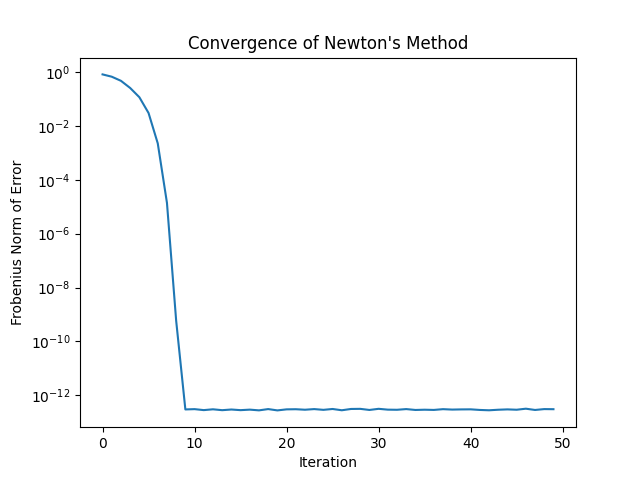
\includegraphics[width=0.6\textwidth]{image/4-1}
                        \caption{牛顿法收敛图像}
                        \label{fig:4-1}
                    \end{figure}\vspace{0.5cm}

            \end{enumerate}

        \item {\color{c1}给定集合$C_i,i=1,2,\cdots,m$为闭凸集,且易于计算投影,考虑投影问题:
            \begin{flalign*}
                \min \quad&\frac12\|x-c\|^2\\\st \quad&x\in C_1\cap C_2\cap\cdots\cap C_m
            \end{flalign*}

            请使用ADMM算法求解此问题,说明是否收敛(无需证明收敛)。}

            \vspace{0.5cm}\textcolor{c2}{解}

            把问题重写为以下形式:
            \begin{flalign*}
                \min_{x,z} \quad&\frac12\|z-c\|^2+\sum_{i=1}^m\mathcal{I}_{C_i}(x_i)\\\st \quad&x_i-z=0,i=1,2,\cdots,m
            \end{flalign*}

            增广Lagrange函数为$L(x,z,\lambda)=\frac12\|z-c\|^2+\sum_{i=1}^m\mathcal{I}_{C_i}(x_i)+\sum_{i=1}^m\lambda_i^{\top}(x_i-z)+\dfrac{\rho}2\sum_{i=1}^m\|x_i-z\|^2$,

            其中$\lambda_i$是Lagrange乘子,$\rho$是正的罚参数。对$x,z$做交替极小化:
            \begin{flalign*}
                x_i^{k+1}=&\argmin_{x_i}\left(\mathcal{I}_{C_i}(x_i)+\lambda_i^{k^{\top}}(x_i-z^k)+\dfrac{\rho}{2}\|x_i-z^{k}\|^2\right)&\\
                =&\argmin_{x_i}\left(\mathcal{I}_{C_i}(x_i)+\lambda_i^{k^{\top}}x_i-\lambda_i^{k^ {\top}}z^k+\dfrac{\rho}{2}\left(\|x_i\|^2+\|z^k\|^2-2x_i^{\top}z^k\right)\right)&\\
                =&\argmin_{x_i}\left(\mathcal{I}_{C_i}(x_i)+\dfrac{\rho}{2}\left(\|x_i\|^2+\left\|z^k-\dfrac1{\rho}\lambda_i^{k^{\top}}\right\|^2-2x_i^{\top}\left(z^k-\dfrac1{\rho}\lambda_i^{k^{\top}}\right)\right)\right)&\\
                =&\argmin_{x_i}\left(\mathcal{I}_{C_i}(x_i)+\dfrac{\rho}{2}\left\|x_i-\left(z^k-\dfrac1{\rho}\lambda_i^{k^{\top}}\right)\right\|\right)&\\
                =&\mathcal{P}_{C_i}\left(z^k-\dfrac1{\rho}\lambda_i^{k^{\top}}\right)&\\
            \end{flalign*}

            $z^{k+1}=\argmin_z\left(\frac12\|z-c\|^2+\sum_{i=1}^m\lambda_i^{k^{\top}}(x_i^{k+1}-z)+\dfrac{\rho}2\sum_{i=1}^m\|x_i^{k+1}-z\|^2\right)\coloneqq \argmin_z \varphi(z)$

            $\nabla \varphi(z)=(z-c)-\sum_{i=1}^m \lambda_i^{k^{\top}}+\rho\sum_{i=1}^m(z-x_i^{k+1})=(1+m\rho)z-c-\sum_{i=1}^k\left(\lambda_i^{k}+\rho x^{k+1}_i\right)=0$

            $\Longrightarrow z^{k+1}=\dfrac{c+\sum\limits_{i=1}^k\left(\lambda_i^{k}+\rho x^{k+1}_i\right)}{1+m\rho},\lambda_i^{k+1}=\lambda_i^k+\tau\rho(x_i^{k+1}-z_i^{k+1}),\tau\in\left(0,\dfrac{1+\sqrt{5}}{2}\right]$

            这个算法是收敛的。\vspace{0.5cm}

        \item {\color{c1}相关系数矩阵的逼近问题的定义为:
            \begin{flalign*}
                \min \quad &\dfrac12\|X-G\|_F^2 \\
                \st \quad& X_{ii}=1, i=1,2,\cdots,n\\
                & X\succeq 0
            \end{flalign*}

            其中自变量$X$取值于对称矩阵空间$S_n$,$G$为给定的实对称矩阵。这个问题在金融领域中有重要的应用。由于误差等因素,根据实际观测得到的相关系数矩阵的估计$G$往往不具有相关系数矩阵的性质(如对角线为$1$,正定性),我们的最终目标是找到一个和$G$最接近的相关系数矩阵$X$。试给出满足如下要求的算法:
            \begin{enumerate}
                \item 对偶近似点梯度法,并给出化简后的迭代公式;
                \item 针对原始问题的ADMM,并给出每个子问题的显式解。
            \end{enumerate}}

            \vspace{0.5cm}\textcolor{c2}{解}

            \begin{enumerate}
                \item Lagrange函数为$L(X,y,Z)=\dfrac12\|X-G\|_F^2-y^{\top}(\diag(X)-\mathbbm{1})-\tr(ZX)$。

                    又$y^{\top}\diag(X)=\tr(\Diag(Y)X)$,其中$Diag(y)$是对角元素为$y$的元素的对角矩阵,

                    故$L(X,y,Z)=\dfrac12\|X-G\|_F^2-\tr(\Diag(Y)X)-\mathbbm{1}^{\top}y-\tr(ZX)$。

                    $\nabla_X L(X,y,Z)=X-G-\Diag(y)-Z=0\Rightarrow X=G+Z+\Diag(Y)$,

                    代回$L(X,y,Z)$得到对偶问题目标函数:
                    \begin{flalign*}
                        g(y,Z)=&\frac12\|G+\Diag(y)+Z-G\|_F^2-\tr(\Diag(y)(G+\Diag(y)+Z))+y^{\top}\mathbbm{1}&\\
                        &-\tr(Z(G+\Diag(y) + Z))&\\
                        =&\frac12\|\Diag(y)+Z\|_F^2-\tr(\Diag(y)G)-\tr(\Diag(y)^2)-\tr(\Diag(y)Z)+y^{\top}\mathbbm{1}&\\
                        &-\tr(ZG)- \tr(Z\Diag(y))-\tr(Z^2)&\\
                        =&-\frac12\|\Diag(y)\|_F^2-\frac12\|Z\|_F^2-\tr(\Diag(y)Z)-\tr(\Diag(y)G)-\tr(ZG)&\\
                        &+y^{\top}\mathbbm{1}&\\
                        =&-\frac12\|\Diag(y)+Z\|_F^2-\tr(G(\Diag(y)+Z))+y^{\top}\mathbbm{1}&\\
                        =&-\frac12\|\Diag(y)+Z+G\|_F^2+\frac12\|G\|_F^2+y^{\top}\mathbbm{1}&
                    \end{flalign*}

                    故对偶问题是$\max\limits_{Z\succeq0,y}\left(-\frac12\|\Diag(y)+Z+G\|_F^2+\frac12\|G\|_F^2+y^{\top} \mathbbm{1}\right)$。

                    等价写为$\min_{y,Z}(f(y,Z)+h(Z))\coloneqq\min_{y,Z}\left(\frac12\|\Diag(y)+Z+G\|_F^2-\mathbbm{1}^{\top}y+\mathcal{I}_{S_+^n}(Z)\right)$

                    此时迭代可写为$(y^{k+1},Z^{k+1})=\prox_{\alpha_k h}\left((y^k,Z^k)-\alpha_k \nabla f(y^k,Z^k)\right)$,$\alpha_k$是步长。

                    先求$\nabla f$,记$\Lambda^k=G+\Diag(y^k)+Z^k,\nabla_y f(y^k,Z^k)=\diag(\Lambda^k)-\mathbbm{1}$,$\nabla_Z f(y^k,Z^k)=\Lambda^k$。

                    记$y^{k+1}_{mid}=y^k-\alpha_k(\diag(\Lambda^k)-\mathbbm{1}),Z^{k+1}_{mid}=Z^k-\alpha_k\Lambda^k$,考虑临近点算子的作用:

                    由于$h$只和$Z$有关,故$y^{k+1}=y^{k+1}_{mid},Z^{k+1}=\prox_{\alpha_k h}(Z^{k+1}_{mid})=\mathcal{P}_{S^n_+}(Z^{k+1}_{mid})$。

                    即$Z^{k+1}_{mid}=V\diag(\lambda_1,\cdots,\lambda_n)V^{\top}$时$Z^{k+1}=V\diag(\max\{0,\lambda_1\},\cdots,\max\{0,\lambda_n\})V^{\top}$。

                    以上给出了一个完整的对偶近似点梯度迭代公式。\vspace{0.5cm}

                \item 把问题重写为以下形式:
                    \begin{flalign*}
                        \min_{X,Z} \quad& \dfrac12\|X-G\|_F^2+\mathcal{I}_{\diag(X)=\mathbbm{1}}(X)+\mathcal{I}_{S^n_+}(Z)\\
                        \st \quad& X-Z=0
                    \end{flalign*}

                    此时增广Lagrange函数为\[L(X,Z,\Lambda)=\dfrac12\|X-G\|_F^2+\mathcal{I}_{\diag(X)=\mathbbm{1}}(X)+\mathcal{I}_{S^n_+}(Z)+\tr(\Lambda^{\top}(X-Z))+\dfrac{\rho}{2}\|X-Z\|_F^2\]

                其中$\Lambda$是Lagrange乘子,$\rho$是正的罚参数。对$X,Z$做交替极小化:

                $X_{ii}^{k+1}$直接取为$1$,只需$\argmin_X \left(\dfrac12\|X-G\|_F^2+\tr(\Lambda^{k^{\top}}(X-Z^k))+\dfrac{\rho}{2}\|X-Z^k\|_F^2\right)$。

                又由于展开式中所有$X_{ij}$均为变量分离形式,故只需按以下方式更新:

                $X_{ij}^{k+1}=\argmin_{X_{ij}}\left(\frac12(X_{ij}-G_{ij})^2+\Lambda^k_{ij}X_{ij}+\frac{\rho}2(X_{ij}-Z^k_{ij})^2\right)=\dfrac{G_{ij}+\rho Z_{ij}^k-\Lambda_{ij}^k}{1+\rho}$
                \begin{flalign*}
                    Z^{k+1}=&\argmin_Z\left(\mathcal{I}_{S^n_+}(Z)+\tr(\Lambda^{\top}(X^{k+1}-Z))+\dfrac{\rho}{2}\|X^{k+1}-Z\|_F^2\right)&\\
                    =&\argmin_Z\left(\mathcal{I}_{S^n_+}(Z)+\dfrac{\rho}{2}\left\|X^{k+1}-Z+ \dfrac{\Lambda^k}{\rho}\right\|_F^2\right)=\mathcal{P}_{S^n_+}\left(X^{k+1}+\dfrac{\Lambda^k}{\rho}\right)&
                \end{flalign*}

                若有特征值分解$X^{k+1}+\dfrac{\Lambda^k}{\rho}=V\diag(\lambda_1,\cdots,\lambda_n)V^{\top}$,则$Z$的更新为:

                $Z^{k+1}=V\diag(\max\{0,\lambda_1\},\cdots,\max\{0,\lambda_n\})V^{\top},\Lambda^{k+1}=\Lambda^k+\rho(X^{k+1}-Z^{k+1})$。\vspace{0.5cm}

            \end{enumerate}

        \item {\color{c1}给定算子$A:\mathbb{R}^n\rightarrow\mathbb{R}^n$,称$A$是单调算子,如果其满足:\[\langle Ax-Ay,x-y \rangle\geq 0,\forall x,y\]

            证明:

            \begin{enumerate}
                \item 给定闭凸函数$f(x)$,次微分算子$\partial f$是单调算子。
                \item 给定闭凸函数$f(x)$,若$f(x)$是$\mu\,$-强凸的,那么$\partial f$是强单调算子,即:\[\langle \partial f(x)-\partial f(y),x-y \rangle\geq \mu\|x-y\|^2,\forall x,y\]
                \item $A$是非扩张的,等价于$\dfrac12(I+A)$是固定非扩张的。
                \item 给定凸函数$f(x)$,且$f(x)$一阶光滑,$\nabla f(x)$是L-Lipchitz连续的。定义$G=I-t\nabla f$,$t\in\left(0,\dfrac1L\right]$
                    \begin{itemize}
                        \item 验证$G$是固定非扩张的。
                        \item 若$f(x)$是$\mu\,$-强凸的,那么$G$是压缩算子,即存在$\rho\in(0,1)$使得\[\|G(x)-G(y)\|\leq\rho\|x-y\|\]
                    \end{itemize}
            \end{enumerate}}


            \vspace{0.5cm}\textcolor{c2}{解}

            \begin{enumerate}
                \item $\forall x,y\in\dom f,g_x\in\partial f(x),g_y\in\partial f(y)$,由次微分定义,有

                    $f(y)\geq f(x)+\langle g_x,y-x \rangle,f(x)\geq f(y)+\langle g_y,x-y \rangle$,

                    相加,$0\geq \langle g_x,y-x \rangle+\langle g_y,x-y \rangle=\langle g_x-g_y,y-x \rangle$,两侧乘$-1$即为单调算子定义。\vspace{0.55cm}

                \item 此时$f(y)\geq f(x)+\langle g_x,y-x \rangle+\dfrac{\mu}{2}\|y-x\|^2,f(x)\geq f(y)+\langle g_y,x-y \rangle+\dfrac{\mu}{2}\|x-y\|^2$

                    仍然相加,$0\geq \langle g_x,y-x \rangle+\langle g_y,x-y \rangle+\mu\|x-y\|^2=-\langle g_y-g_x,y-x \rangle+\mu\|x-y\|^2$,

                    $\Rightarrow \langle g_y-g_x,y-x \rangle\geq\mu\|x-y\|^2$,即为强单调算子定义。\vspace{0.5cm}

                \item $\Longrightarrow$:记$T=\frac12 (I+A),u=Tx,v=Ty,A=2T-I,\|(2T-I)x-(2T-I)y\|^2\leq\|x-y\|^2$,

                    即$\|2(u-v)-(x-y)\|^2\leq\|x-y\|^2\Rightarrow 4\|u-v\|^2-4\langle u-v,x-y \rangle+\|x-y\|^2\leq\|x-y\|^2$,

                    $\Rightarrow \|u-v\|^2\leq\langle u-v,x-y \rangle$,即$\|Tx-Ty\|^2\leq\langle Tx-Ty,x-y \rangle$,故$T$固定非扩张。

                    \vspace{0.25cm}$\Longleftarrow$:由$\|u-v\|^2\leq\langle u-v,x-y \rangle$有$4\|u-v\|^2\leq4\langle u-v,x-y \rangle$,此时

                    $\Rightarrow 4\|u-v\|^2-4\langle u-v,x-y \rangle+\|x-y\|^2\leq\|x-y\|^2\Rightarrow\|2(u-v)-(x-y)\|^2\leq\|x-y\|^2$

                    $\Rightarrow \|(2T-I)x-(2T-I)y\|^2=\|Ax-Ay\|^2\leq\|x-y\|^2$,即$A$非扩张。\vspace{0.5cm}

                \item
                    \begin{itemize}
                        \item 由$\nabla f$是L-Lipchitz连续的,有$\langle \nabla f(x)-\nabla f(y),x-y \rangle\geq\dfrac1L\|\nabla f(x)-\nabla f(y)\|^2$。
                            记$H=2G-I=I-2t\nabla f$,则有
                            \begin{flalign*}
                                \|H(x)-H(y)\|^2=&\|x-y-2t(\nabla f(x)-\nabla f(y))\|^2&\\
                                =&\|x-y\|^2-4t\langle \nabla f(x)-\nabla f(y),x-y \rangle+4t^2\|\nabla f(x)-\nabla f(y)\|^2&\\
                                \leq& \|x-y\|^2-\dfrac{4t}L\|\nabla f(x)-\nabla f(y)\|^2+4t^2\|\nabla f(x)-\nabla f(y)\|^2&\\
                                =&\|x-y\|^2+4(t^2-\dfrac{t}L)\|\nabla f(x)-\nabla f(y)\|^2\leq\|x-y\|^2
                            \end{flalign*}

                            故$H$是非扩张的,进而$G$是固定非扩张的。\vspace{0.25cm}

                        \item 由$f$是$\mu\,$-强凸的,有$\langle \nabla f(x)-\nabla f(y),x-y \rangle\geq\mu\|x-y\|^2$。
                            \begin{flalign*}
                                \|G(x)-G(y)\|=&\|x-y-t(\nabla f(x)-\nabla f(y))\|^2&\\
                                =&\|x-y\|^2-2t\langle \nabla f(x)-\nabla f(y),x-y \rangle+t^2\|\nabla f(x)-\nabla f(y)\|^2&\\
                                \leq&\|x-y\|^2-2t\mu\|x-y\|^2+t^2 L^2\|x-y\|^2&\\
                                =&(L^2 t^2-2\mu t+1)\|x-y\|^2\leq\|x-y\|^2
                            \end{flalign*}

                            故$G$是压缩算子。
                    \end{itemize}
            \end{enumerate}

    \end{enumerate}



\end{document}